\documentclass{article}

\usepackage{tikz}

\begin{document}

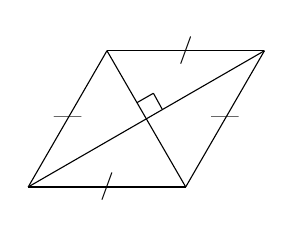
\begin{tikzpicture}
  % Losange
  \draw (0,0) -- (1,1.73);
  \draw (1,1.73)-- (3,1.73);
  \draw (2,0)-- (3,1.73); 
  \draw (0,0)-- (2,0);
  % Diagonales
  \draw (0,0)-- (3,1.73);
  \draw (1,1.73)-- (2,0);
  % Angle droit
  \draw  (1.38,1.07)-- (1.59,1.19);
  \draw  (1.59,1.19)-- (1.7,0.99);
  %  Marques sur les bords
  \draw (2,1.73) node{$/$};
  \draw  (2.5,0.87) node{---};
  \draw  (1,0) node{$/$};
  \draw  (0.5,0.87) node{---};
\end{tikzpicture}

\end{document}
